% !TeX root = ../main.tex
\section{Прохождение шума через БВЧ РПУ}

\subsection{Решение задачи №1-1}

На вход приёмника подключён эквивалент согласованной антенны, находящийся при стандартной температуре $T_0 = 293$~К. Мощность шума на выходе блока высокой частоты (БВЧ) составляет $P_{\text{ш.вых}} = 20 \cdot 10^{-9}$~Вт. Шумовая полоса приёмного тракта равна $\Pi_{\text{ш}} = 2$~МГц, а коэффициент усиления проходной мощности БВЧ составляет $K_{p\text{ БВЧ}} = 60$~дБ.
Требуется определить мощность приведённого ко входу собственного шума приёмника $P_{\text{ш.соб.ном}}'$.

\paragraph{Решение.}
Переведём коэффициент усиления проходной мощности БВЧ из децибел в разы:
\begin{equation}
    K_p = 10^{\frac{K_{p\text{, дБ}}}{10}} = 10^{\frac{60}{10}} = 10^6.
\end{equation}

Полная мощность шума на входе БВЧ складывается из мощности шума антенны $P_{\text{ант.вх}}$ и приведённой мощности собственного шума приёмника $P_{\text{ш.соб.ном}}'$:
\begin{equation}
    P_{\text{ш.вх}} = P_{\text{ант.вх}} + P_{\text{ш.соб.ном}}'.
\end{equation}

Мощность теплового шума согласованной антенны при температуре $T_A = T_0 = 293$~К определяется формулой Найквиста:
\begin{equation}
    P_{\text{ант.вх}} = k T_0 \Pi_{\text{ш}},
\end{equation}
где $k = 1{,}38 \cdot 10^{-23}$~Дж/К — постоянная Больцмана.

Связь между мощностью шума на входе и выходе БВЧ задаётся через коэффициент передачи мощности:
\begin{equation}
    P_{\text{ш.вх}} = \frac{P_{\text{ш.вых}}}{K_p}.
\end{equation}

Тогда мощность приведённого ко входу собственного шума приёмника принимает вид:
\begin{equation}
    P_{\text{ш.соб.ном}}' = \frac{P_{\text{ш.вых}}}{K_p} - k T_0 \Pi_{\text{ш}}.
\end{equation}

Подставляя числовые значения, получаем:
\begin{equation}
    P_{\text{ш.соб.ном}}' = \frac{20 \cdot 10^{-9}}{10^6} - 1{,}38 \cdot 10^{-23} \cdot 293 \cdot 2 \cdot 10^6 = 2{,}0 \cdot 10^{-14} - 8{,}087 \cdot 10^{-15} \approx 1{,}191 \cdot 10^{-14}\text{ Вт}.
\end{equation}

\noindent\textbf{Ответ:} $P_{\text{ш.соб.ном}}' \approx 1{,}191 \cdot 10^{-14}$~Вт ($11{,}91$~фВт).

\begin{figure}[h!]
    \centering
    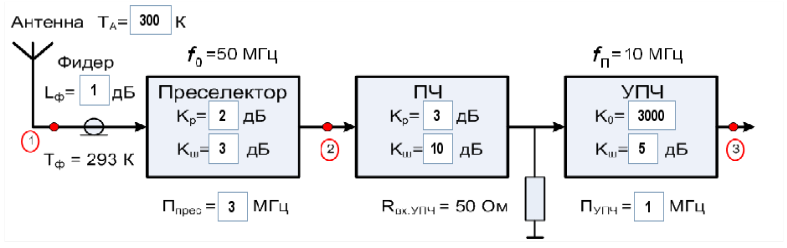
\includegraphics[width=0.95\linewidth]{exports_fig/scheme_bvch.png}
    \caption{Схема БВЧ для лабораторной работы}
    \label{fig:scheme_bvch}
\end{figure}
Для аналитического расчёта сквозных характеристик тракта перейдём от логарифмических единиц (децибел) к линейным безразмерным величинам по базовому соотношению $K = 10^{K_{[\text{дБ}]} / 10}$. В результате получаем следующие параметры звеньев цепи:
\begin{align*}
    L_\Phi &= 10^{1/10} \approx 1{,}26, & K_{p\Phi} &= \frac{1}{L_\Phi} \approx 0{,}8, \\
    K_{p\text{ прес}} &= 10^{2/10} \approx 1{,}58, & K_{\text{ш прес}} &= 10^{3/10} \approx 1{,}99, \\
    K_{p\text{ ПЧ}} &= 10^{3/10} \approx 1{,}99, & K_{\text{ш ПЧ}} &= 10^{10/10} = 10, \\
    K_0 &= 3000, & K_{\text{ш УПЧ}} &= 10^{5/10} \approx 3{,}16.
\end{align*}

Поскольку фидер представляет собой пассивный четырехполюсник с потерями при физической температуре $T_\Phi = 293$~К, его коэффициент шума определяется затуханием $L_\Phi$ и термодинамической температурой:
\begin{equation}
    K_{\text{ш }\Phi} = 1 + \frac{T_\Phi}{T_0}(L_\Phi - 1) = 1 + \frac{293}{293}(1{,}26 - 1) = 1{,}26.
\end{equation}

Коэффициент передачи по мощности несогласованного пассивного фидера обратно пропорционален его коэффициенту шума при равенстве температур:
\begin{equation}
    K_{p\Phi} = \frac{1}{K_{\text{ш }\Phi}} = \frac{1}{1{,}26} \approx 0{,}8.
\end{equation}

Сквозной коэффициент шума тракта БВЧ, представляющего собой каскадное соединение линейных четырехполюсников, определяется обобщённой формулой Фрииса:
\begin{align}
    K_{\text{ш БВЧ}} &= K_{\text{ш }\Phi} + \frac{K_{\text{ш прес}} - 1}{K_{p\Phi}} + \frac{K_{\text{ш ПЧ}} - 1}{K_{p\Phi} K_{p\text{ прес}}} + \frac{K_{\text{ш УПЧ}} - 1}{K_{p\Phi} K_{p\text{ прес}} K_{p\text{ ПЧ}}} \\
    &= 1{,}26 + \frac{1{,}99 - 1}{0{,}8} + \frac{10 - 1}{0{,}8 \cdot 1{,}58} + \frac{3{,}162 - 1}{0{,}8 \cdot 1{,}58 \cdot 1{,}99} \approx 10{,}48.
\end{align}

Зная результирующий коэффициент шума, определим эквивалентную шумовую температуру блока высокой частоты:
\begin{equation}
    T_{\text{ш БВЧ}} = T_0 \left( K_{\text{ш БВЧ}} - 1 \right) = 293 \cdot (10{,}48 - 1) \approx 2774{,}7\text{ К}.
\end{equation}

Полная шумовая температура радиоприёмного устройства с учётом эквивалентной температуры согласованной антенны $T_A = 300$~К принимает значение:
\begin{equation}
    T_{\Sigma\text{ РПУ}} = T_A + T_{\text{ш БВЧ}} = 300 + 2774{,}7 = 3074{,}7\text{ К}.
\end{equation}

Спектральная плотность мощности (СПМ) суммарного шума, приведённого к антенному входу приемника, вычисляется через фундаментальное соотношение Найквиста:
\begin{equation}
    G_{\Sigma\text{ ном}}' = k T_{\Sigma\text{ РПУ}} = 1{,}38 \cdot 10^{-23} \cdot 3074{,}7 \approx 4{,}25 \cdot 10^{-20}\text{ Вт/Гц} = 4{,}25 \cdot 10^{-14}\text{ Вт/МГц}.
\end{equation}

\begin{figure}[h!]
    \centering
    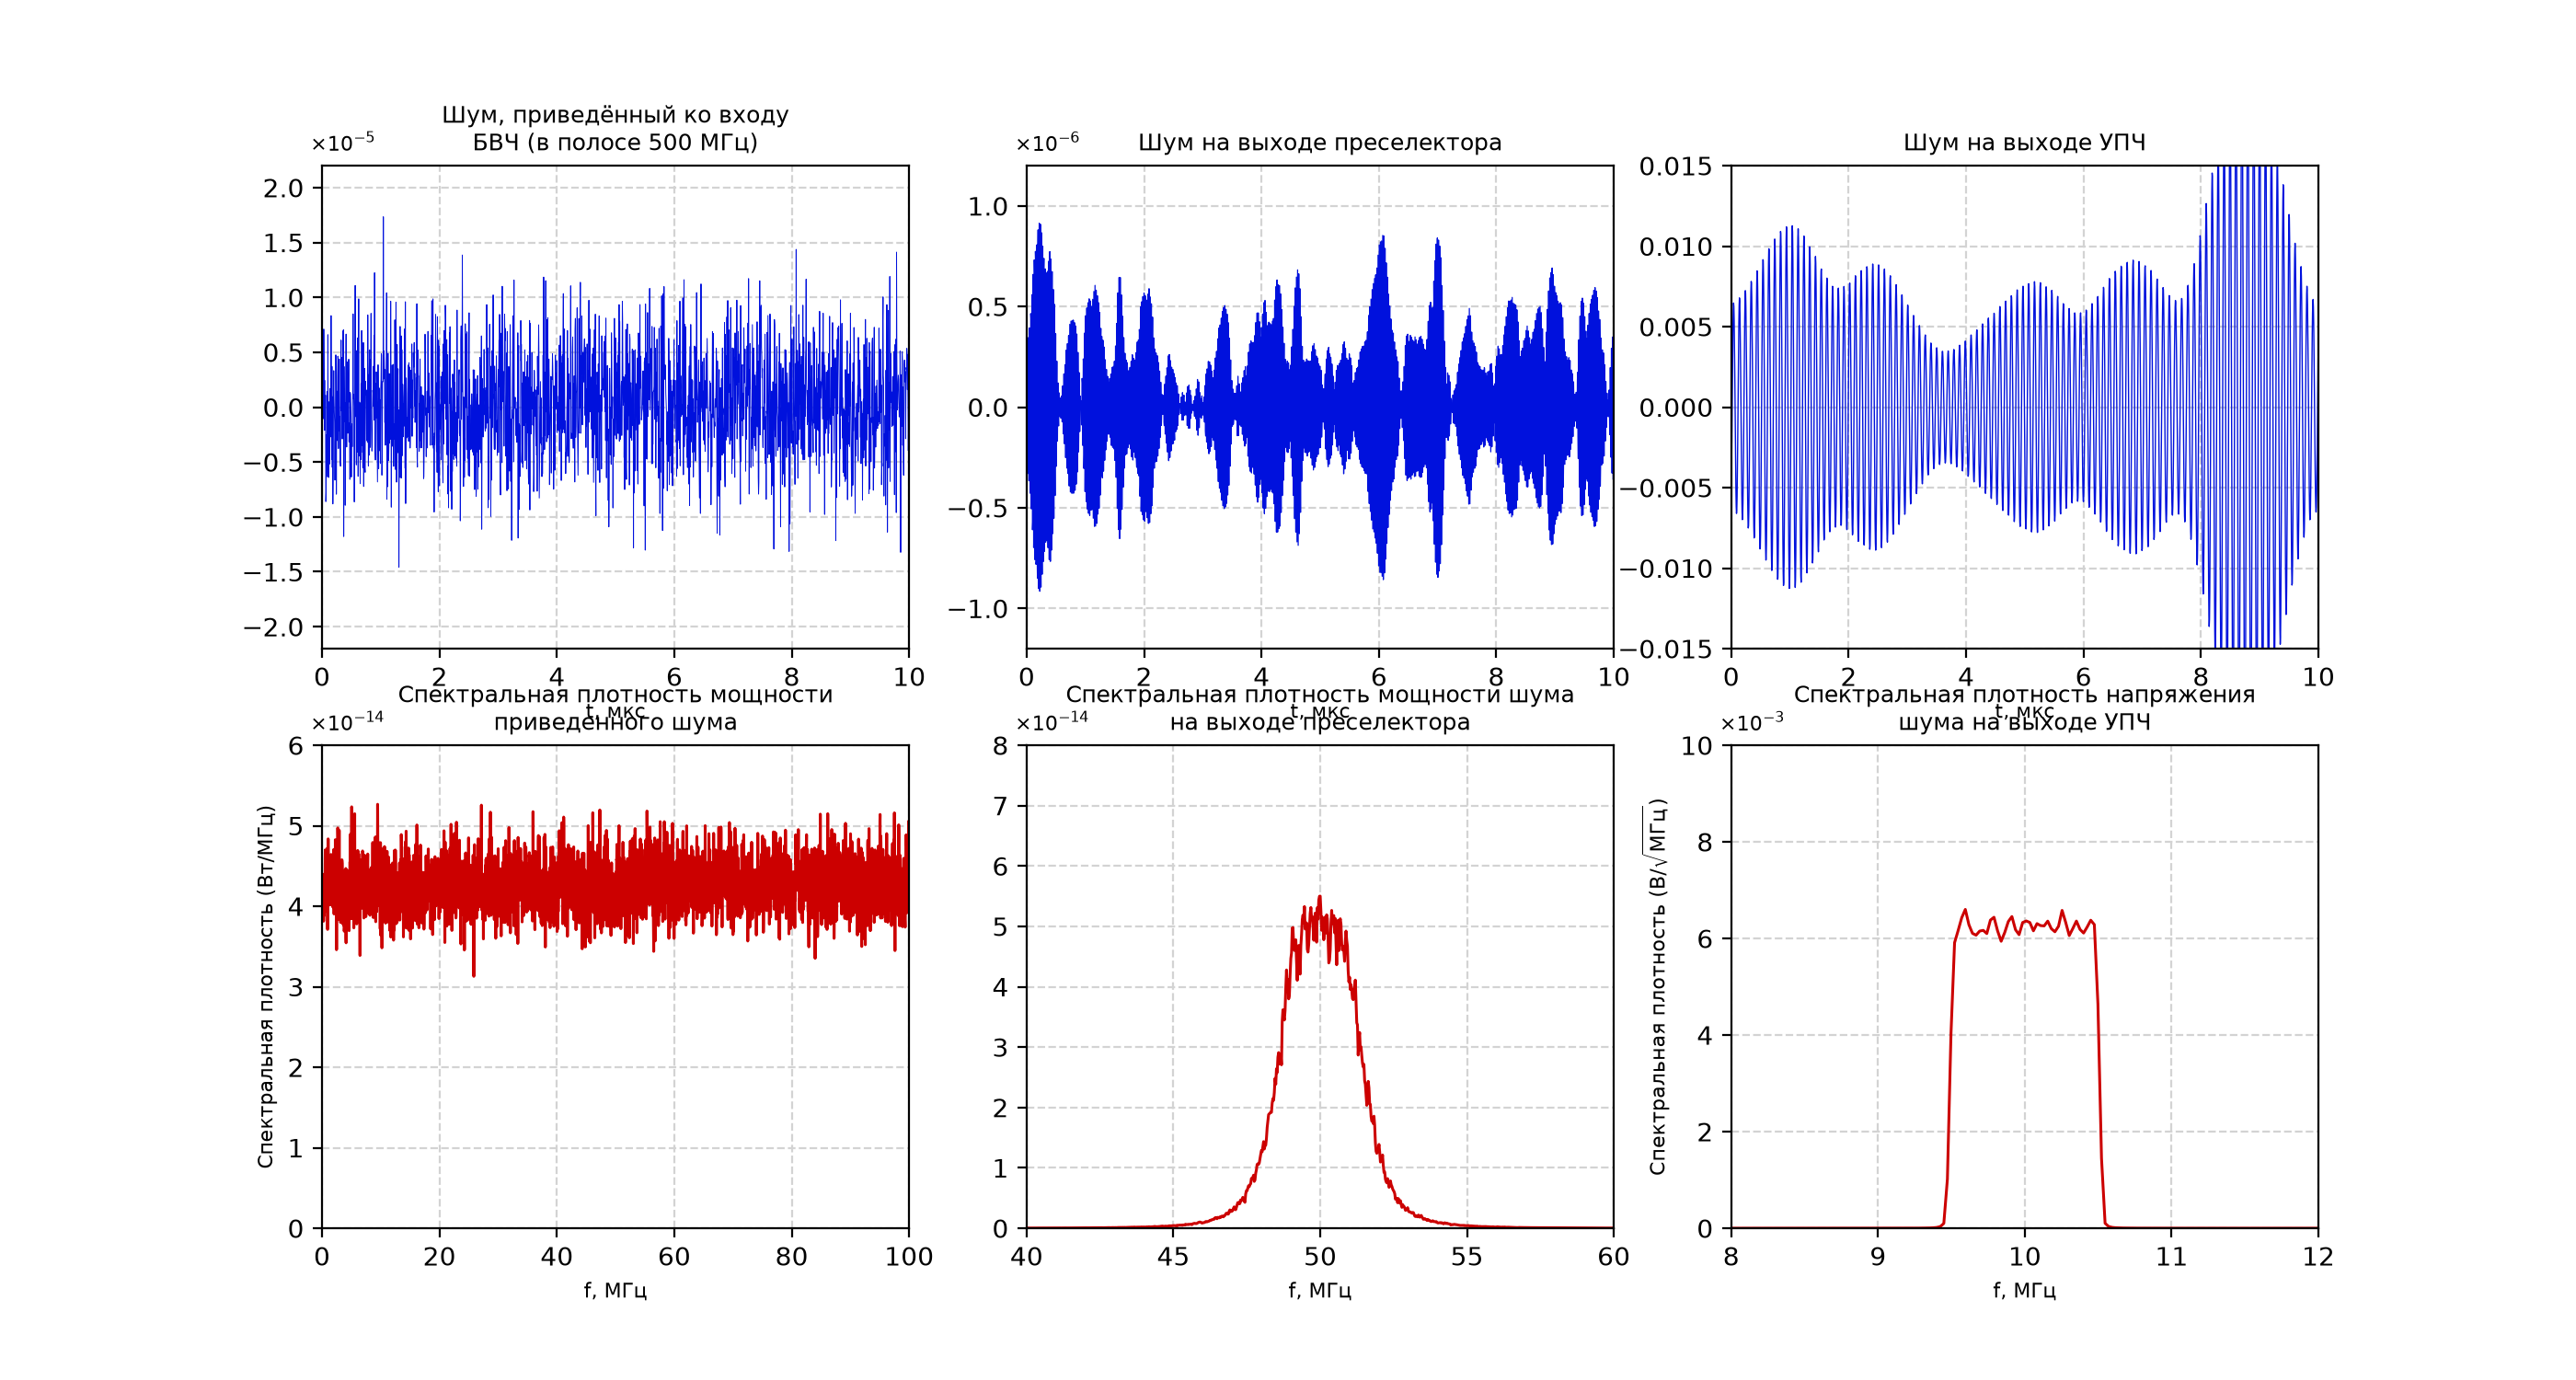
\includegraphics[width=0.98\linewidth]{exports_fig/pic1.png}
    \caption{Характеристики квазигармонического шума и спектральные плотности в контрольных сечениях тракта БВЧ}
    \label{fig:bvch_simulation_base}
\end{figure}

По результатам численного моделирования в среде с объёмом выборки более $10^6$ отсчётов измеренное на виртуальном приборе значение спектральной плотности мощности приведённого шума составило $4{,}26 \cdot 10^{-14}$~Вт/МГц ($4{,}26 \cdot 10^{-20}$~Вт/Гц). Полученное значение практически полностью совпадает с теоретическим расчётом ($4{,}257 \cdot 10^{-20}$~Вт/Гц), а погрешность не превышает сотых долей процента и вызвана округлением константы Больцмана и конечностью интервала усреднения спектра.

\subsection{Измерение эквивалентной шумовой температуры БВЧ}

На первом этапе задаётся исходная температура согласованного источника $T_{A1} = T_0 = 293$~К. Теоретическое значение суммарной спектральной плотности мощности шума на входе тракта составляет:
\begin{equation}
    G_{ш\Sigma}^{(1)} = k \left( T_0 + T_{ш\text{ БВЧ}} \right) = 1{,}38 \cdot 10^{-23} \cdot (293 + 2774{,}7) \approx 4{,}24 \cdot 10^{-20}\text{ Вт/Гц}.
\end{equation}

\begin{figure}[H]
    \centering
    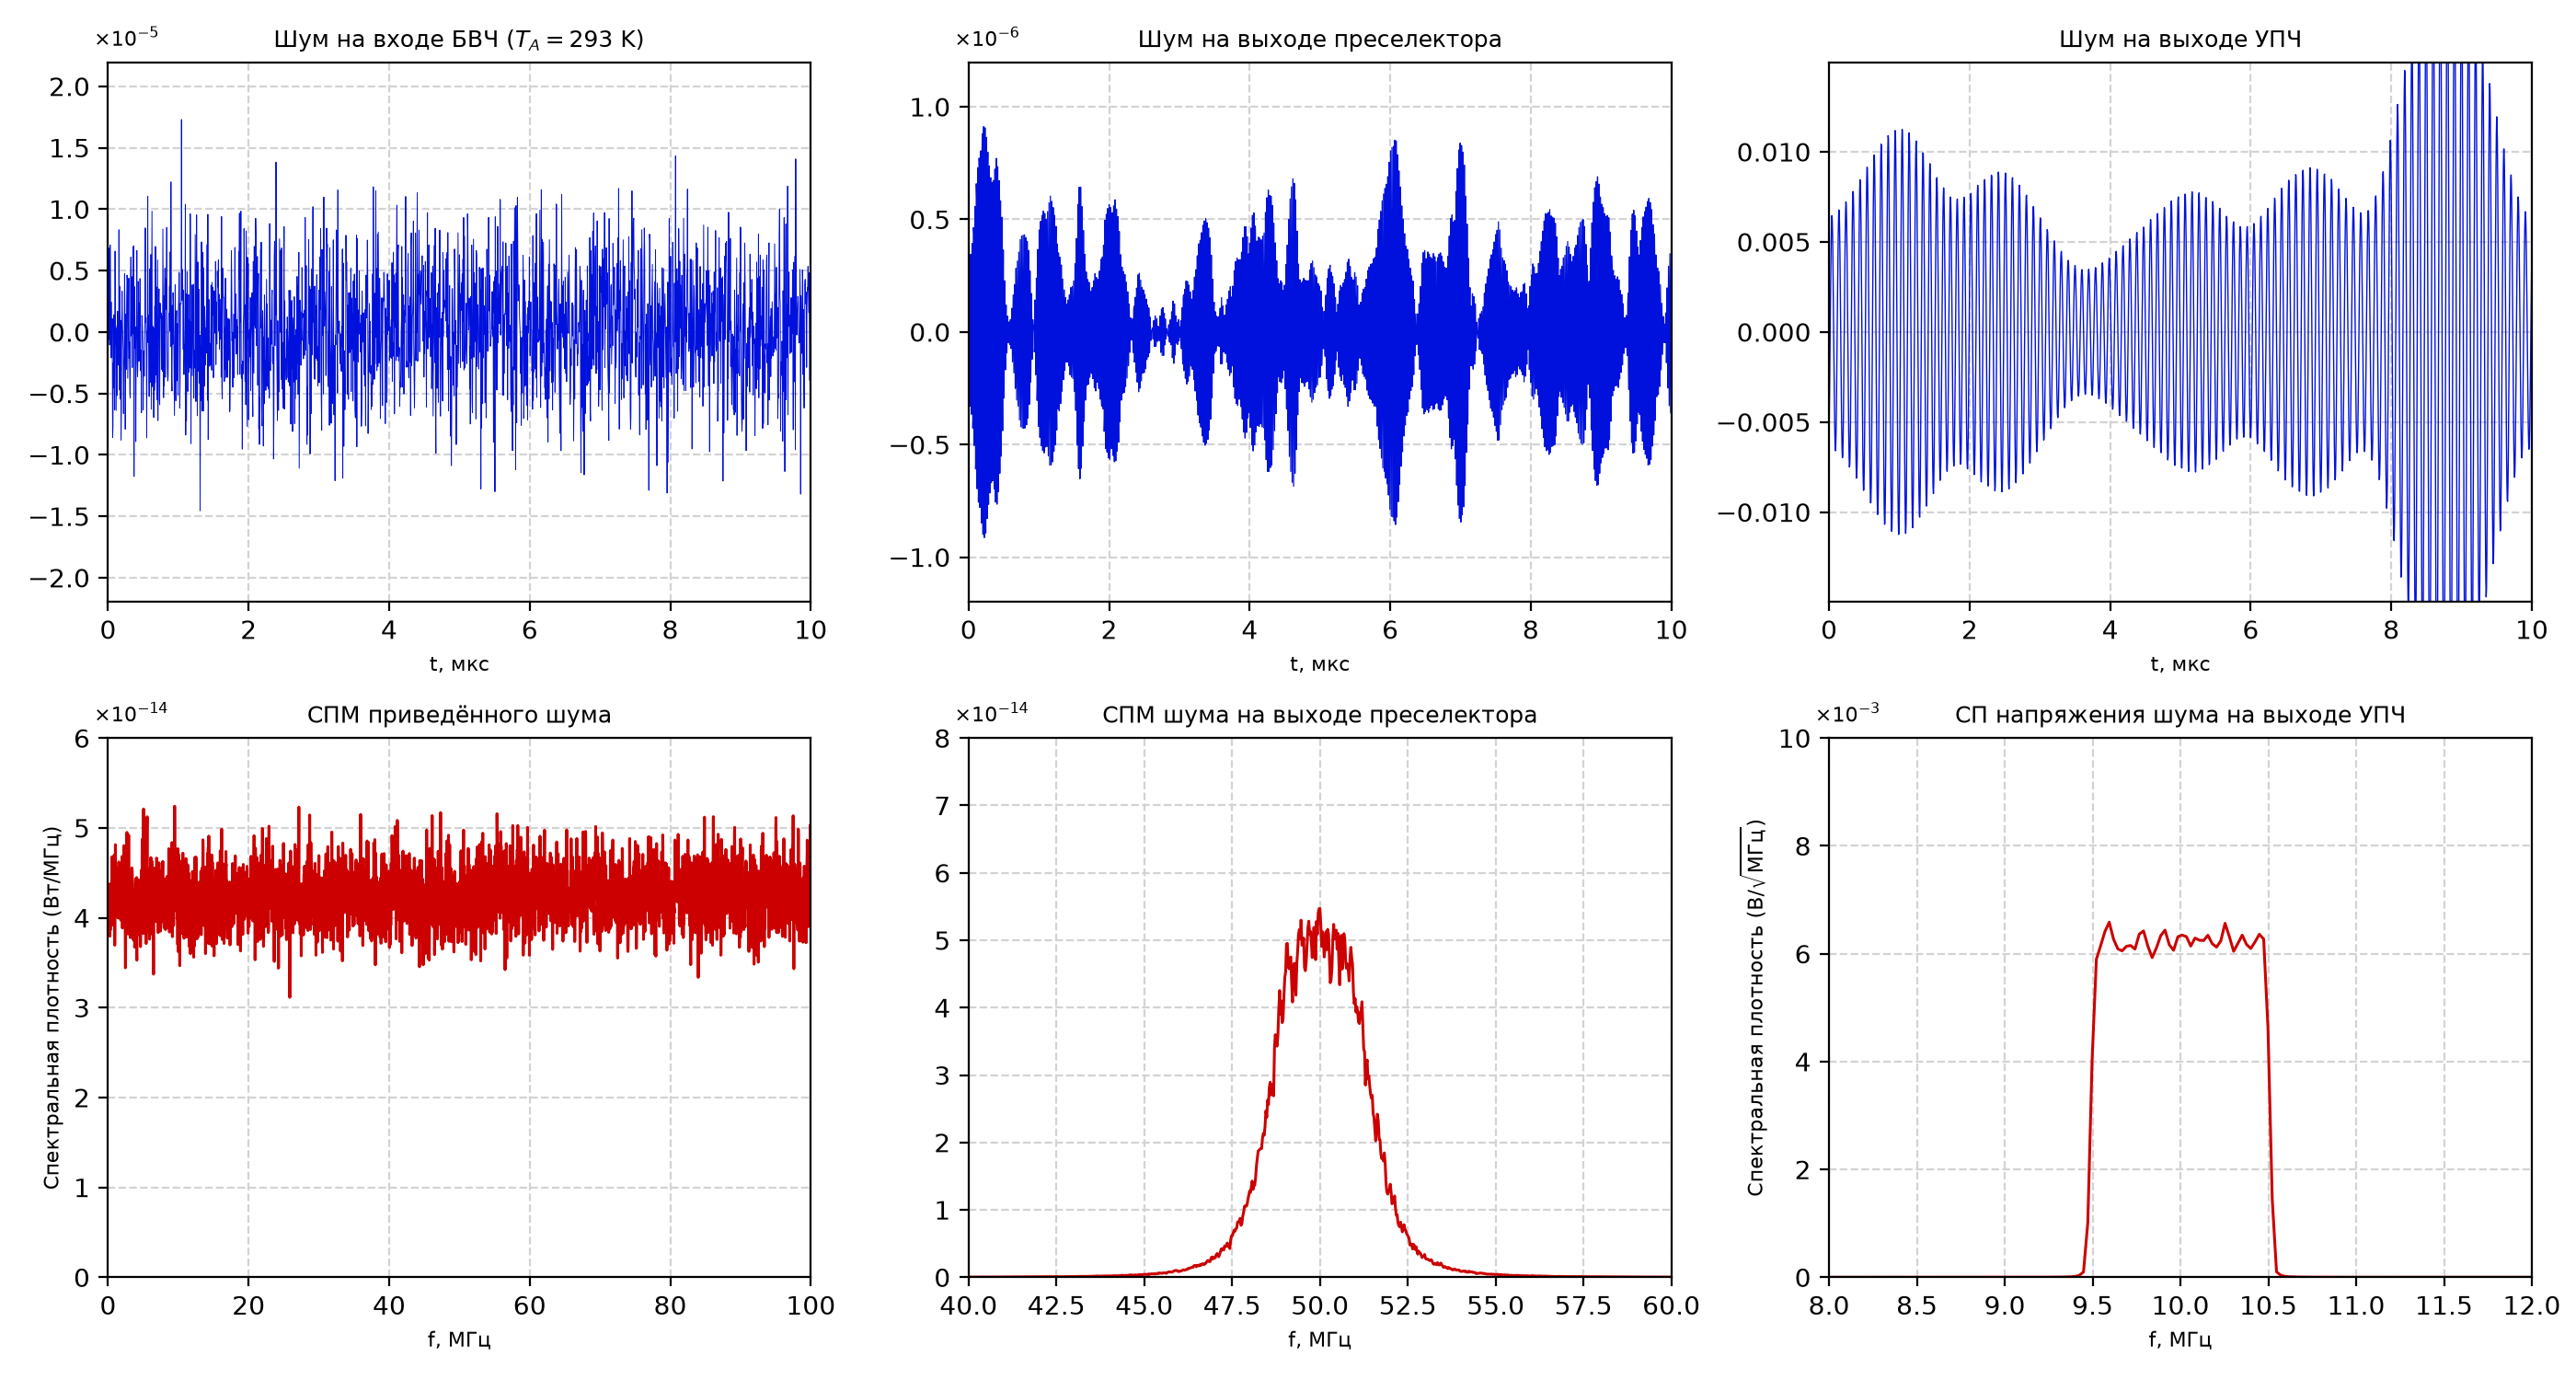
\includegraphics[width=0.98\linewidth]{exports_fig/pic2.png}
    \caption{Характеристики шума в тракте БВЧ при температуре антенны $T_{A1} = 293$~К}
    \label{fig:noise_temp_initial}
\end{figure}

На втором этапе температура антенны повышается до некоторого значения $T_{A2} > T_0$ такого, чтобы суммарная спектральная плотность мощности приведённого ко входу шума возросла ровно в два раза:
\begin{equation}
    G_{ш\Sigma}^{(2)} = 2 \, G_{ш\Sigma}^{(1)} = k \left( T_{A2} + T_{ш\text{ БВЧ}} \right).
\end{equation}

Подставляя численные значения, получаем требуемый уровень СПМ $G_{ш\Sigma}^{(2)} \approx 8{,}487 \cdot 10^{-20}$~Вт/Гц, чему соответствует эквивалентная температура антенны $T_{A2} = 3371$~К.

\begin{figure}[H]
    \centering
    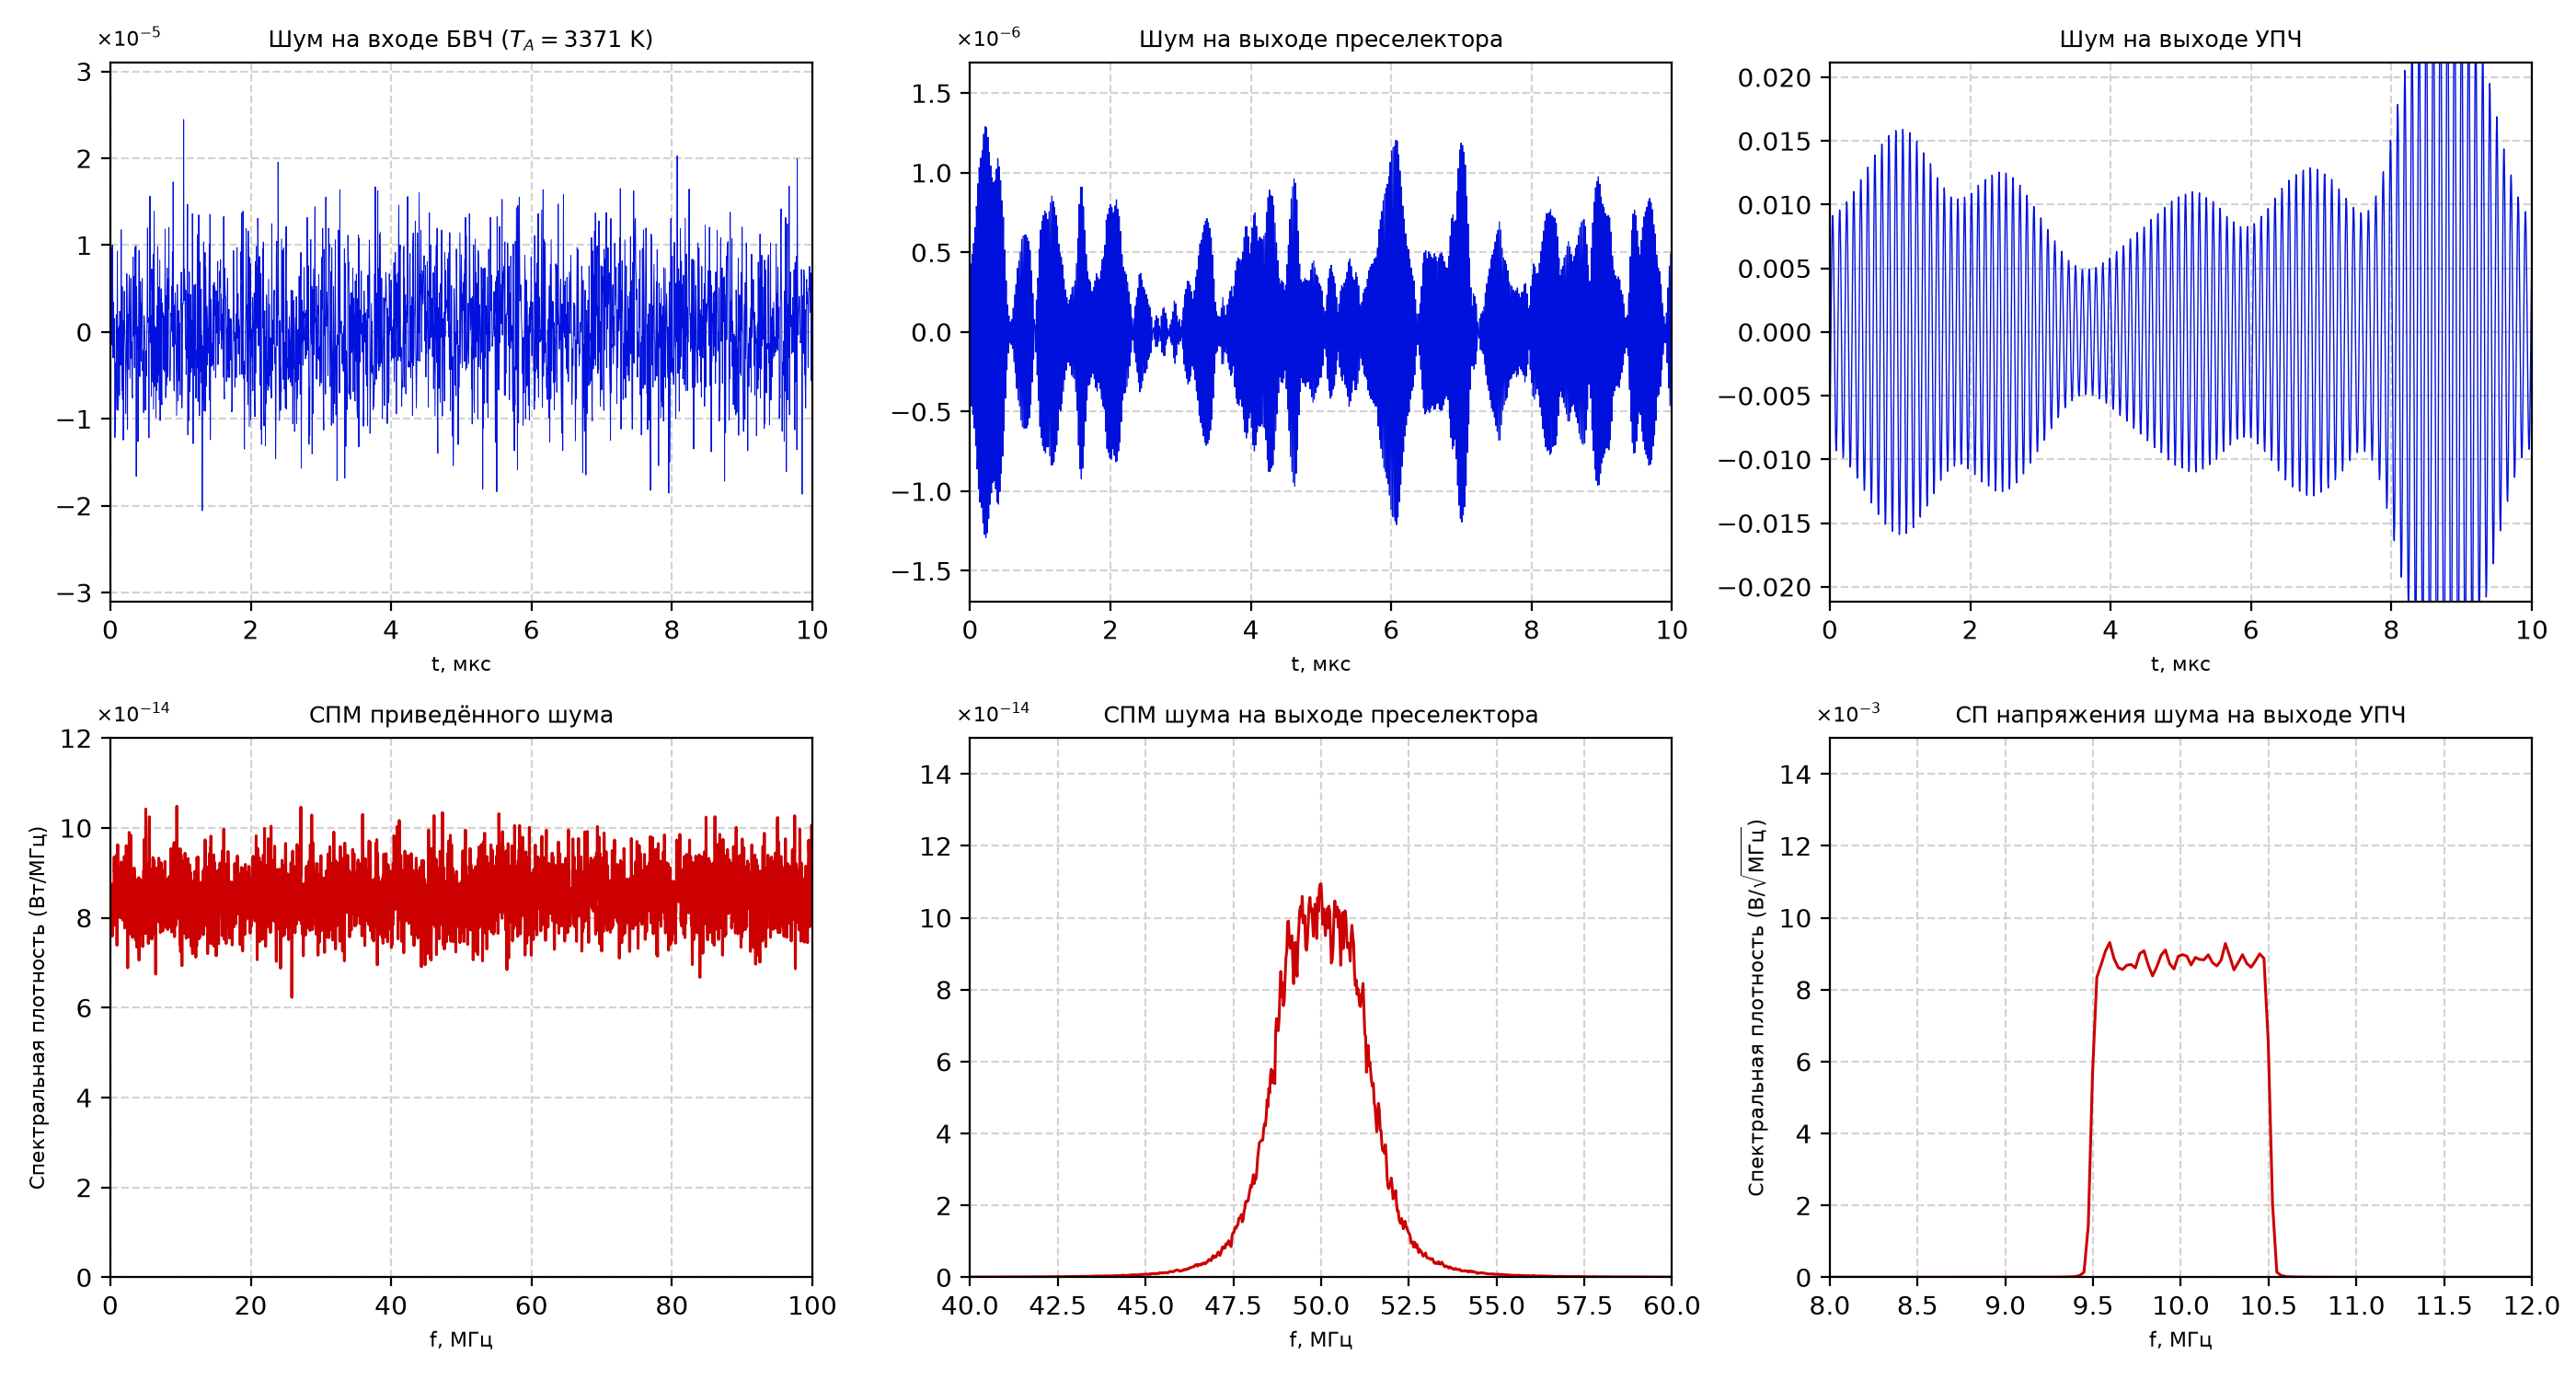
\includegraphics[width=0.98\linewidth]{exports_fig/pic3.png}
    \caption{Характеристики шума в тракте БВЧ при подобранной температуре $T_{A2} = 3371$~К}
    \label{fig:noise_temp_doubled}
\end{figure}

Используя условие удвоения мощности ($T_{A2} + T_{ш\text{ БВЧ}} = 2(T_0 + T_{ш\text{ БВЧ}})$), определяем экспериментальную шумовую температуру исследуемого блока высокой частоты:
\begin{equation}
    T_{ш\text{ БВЧ}} = T_{A2} - 2 T_0 = 3371 - 2 \cdot 293 = 2785\text{ К}.
\end{equation}

Полученное по результатам измерений на модели значение $2785$~К находится в строгом согласии с ранее рассчитанной теоретической величиной $2774{,}7$~К. Незначительное расхождение (менее $0{,}4\%$) обусловлено шагом дискретной подстройки температуры на виртуальном стенде и погрешностью спектрального оценивания.

\subsection{Оценка влияния параметров БВЧ на чувствительность РПУ}
Чувствительность радиоприёмного устройства напрямую определяется уровнем шума, приведённого к его входу: чем меньше спектральная плотность мощности приведённого шума $G_{\Sigma\text{ ном}}' = k(T_A + T_{\text{ш БВЧ}})$, тем более слабый сигнал приёмник способен обнаружить. Для оценки роли отдельных каскадов тракта проведено исследование влияния коэффициента усиления преселектора, коэффициента шума смесителя (ПЧ) и потерь во входном фидере при температуре антенны $T_A = 300$~К.

\textbf{Пункт А.} Подберём такое значение коэффициента передачи преселектора $K_{p\text{ прес}}$, при котором спектральная плотность мощности приведённого шума уменьшается ровно в 2 раза по сравнению с номинальным режимом (до величины $G_{\Sigma}' \approx 2{,}11 \cdot 10^{-14}$~Вт/МГц). По результатам подбора на модели получено $K_{p\text{ прес}} = 6{,}75$~дБ ($K_{p\text{ прес}} \approx 4{,}73$).

\begin{figure}[h!]
    \centering
    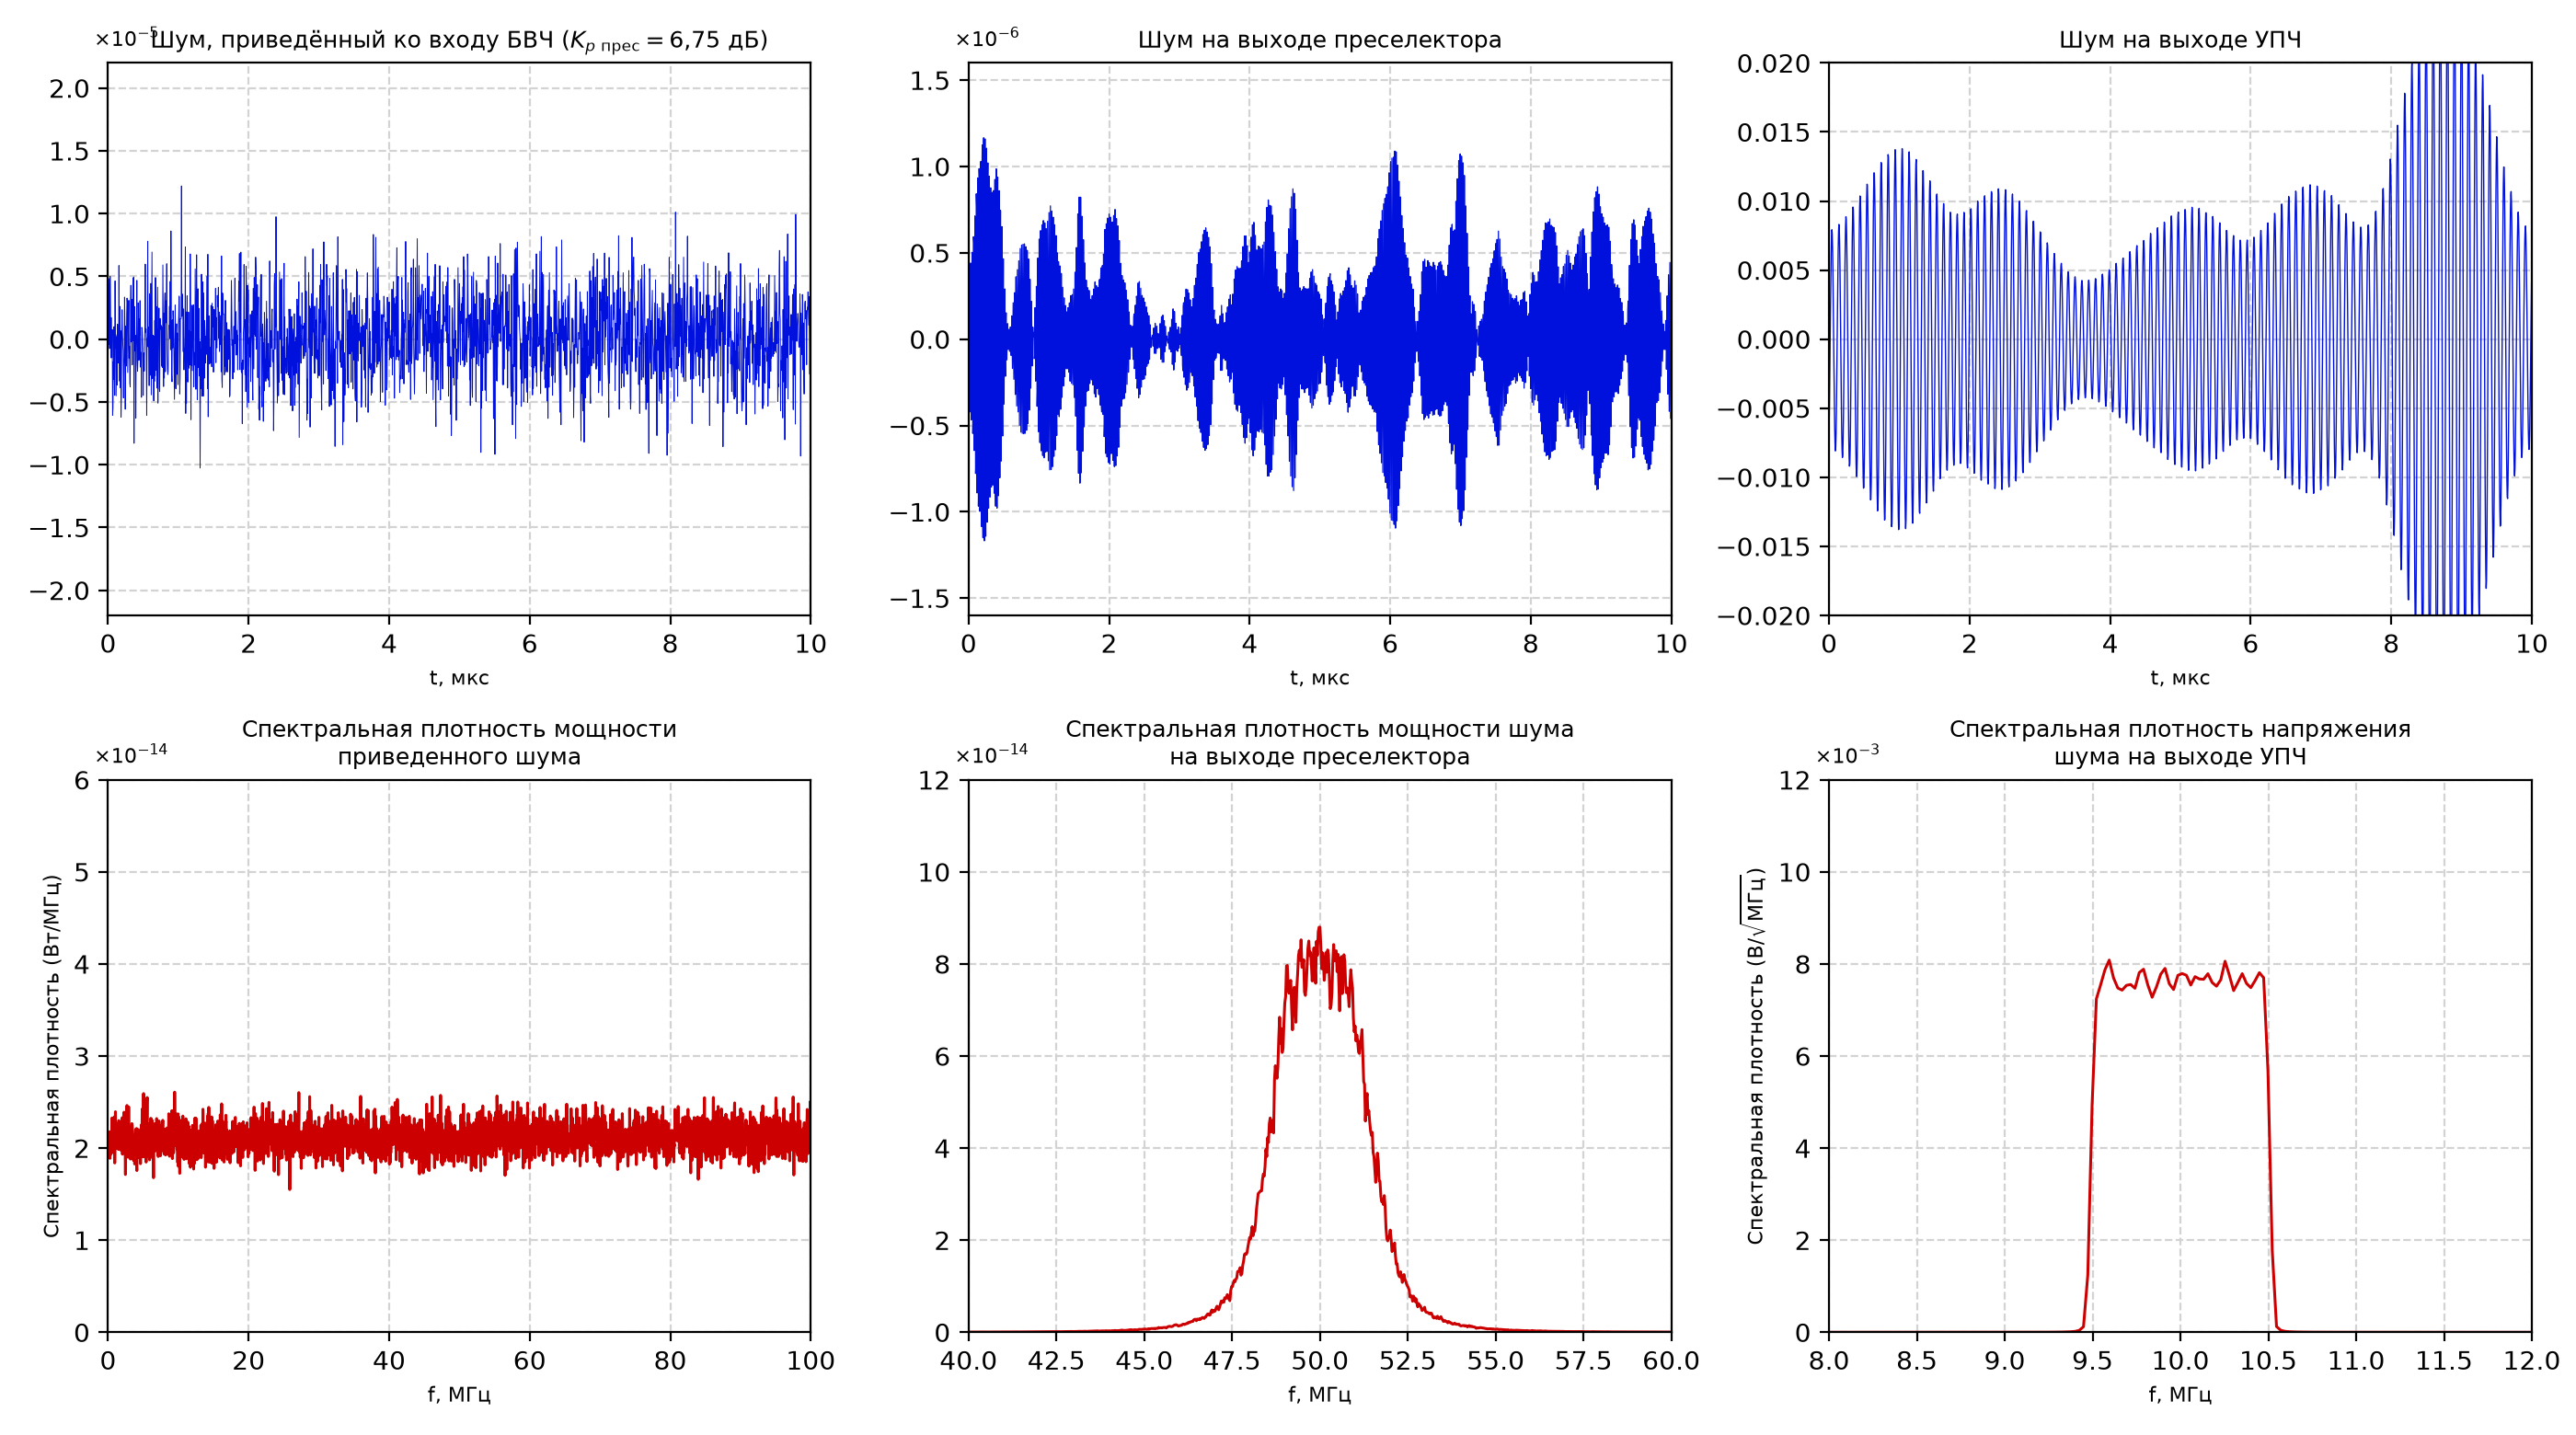
\includegraphics[width=0.98\linewidth]{exports_fig/pic4.png}
    \caption{Характеристики шума в тракте БВЧ при подобранном коэффициенте передачи $K_{p\text{ прес}} = 6{,}75$~дБ}
    \label{fig:sens_kp_pres}
\end{figure}

Увеличение коэффициента передачи первого каскада приводит к значительному ослаблению влияния шумов последующих каскадов (ПЧ и УПЧ), так как по формуле Фрииса их шумовые температуры делятся на произведение коэффициентов передачи предшествующих звеньев. В результате сквозная шумовая температура тракта падает, СПМ приведённого шума снижается вдвое, а чувствительность приёмника возрастает.

\textbf{Пункт Б.} Восстановим исходный коэффициент передачи мощности преселектора $K_{p\text{ прес}} = 2$~дБ ($K_{p\text{ прес}} \approx 1{,}58$) и подберём такое значение коэффициента шума смесителя $K_{\text{ш ПЧ}}$, при котором спектральная плотность мощности приведённого шума также уменьшается в 2 раза по сравнению с номинальным режимом ($G_{\Sigma}' \approx 2{,}12 \cdot 10^{-14}$~Вт/МГц).

\begin{figure}[H]
    \centering
    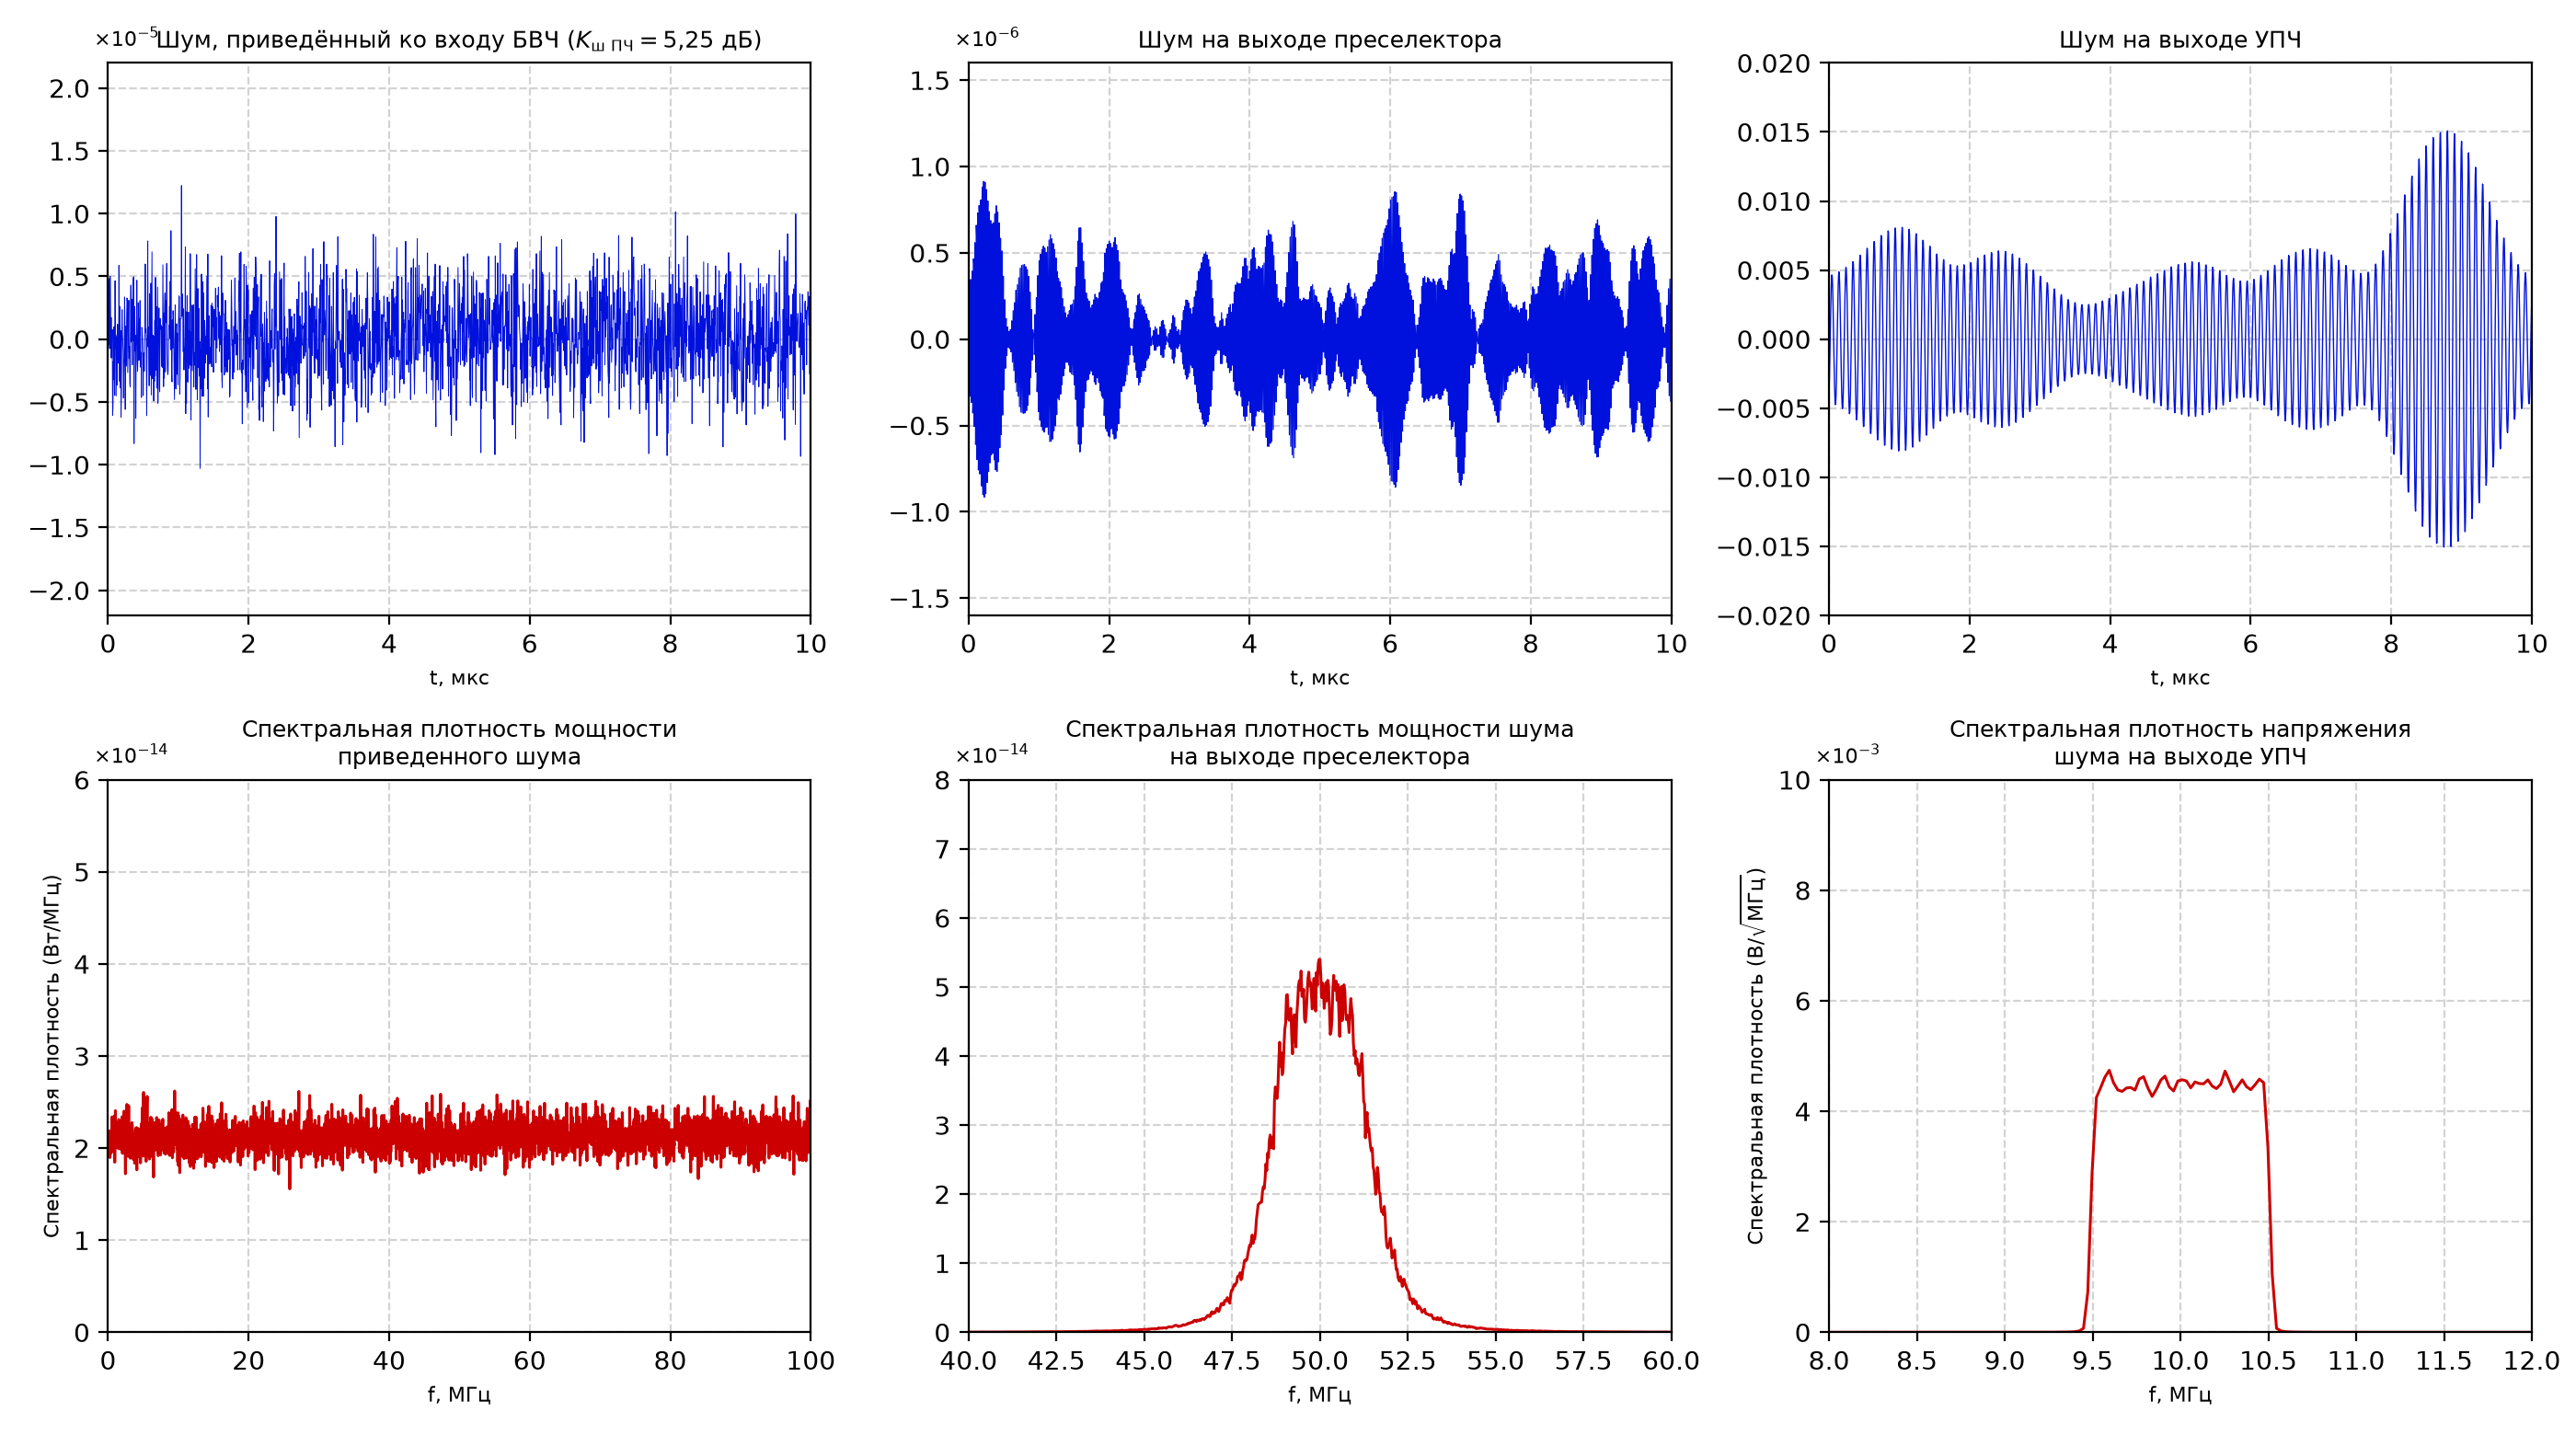
\includegraphics[width=0.98\linewidth]{exports_fig/pic5.png}
    \caption{Характеристики шума в тракте БВЧ при подобранном коэффициенте шума ПЧ $K_{\text{ш ПЧ}} = 5{,}25$~дБ}
    \label{fig:sens_kn_pch}
\end{figure}

В структуре тракта преобразователь частоты вносит существенный собственный шум ($K_{\text{ш ПЧ}} = 10$~дБ). Из-за сравнительно небольшого усиления преселектора ($2$~дБ) шумовой вклад смесителя $\frac{K_{\text{ш ПЧ}} - 1}{K_{p\Phi} K_{p\text{ прес}}}$ был доминирующим. Снижение коэффициента шума смесителя до $5{,}25$~дБ уменьшает результирующую шумовую температуру тракта и приводит к двукратному повышению чувствительности системы. При этом спектральная плотность шума на выходе преселектора остаётся прежней, так как смеситель расположен дальше по тракту.

\textbf{Пункт В.} Оценим возможное повышение чувствительности приёмника за счёт устранения потерь в антенно-фидерном тракте. Для этого сопоставим значение спектральной плотности мощности приведённого шума при номинальных потерях фидера $L_\Phi = 1$~дБ ($K_{p\Phi} \approx 0{,}8$) и в случае идеального согласованного фидера без потерь $L_\Phi = 0$~дБ ($K_{p\Phi} = 1$).

По результатам моделирования при $L_\Phi = 0$~дБ спектральная плотность мощности приведённого ко входу шума снизилась до величины $G_{\Sigma}' \approx 3{,}39 \cdot 10^{-14}$~Вт/МГц ($3{,}39 \cdot 10^{-20}$~Вт/Гц).

\begin{figure}[H]
    \centering
    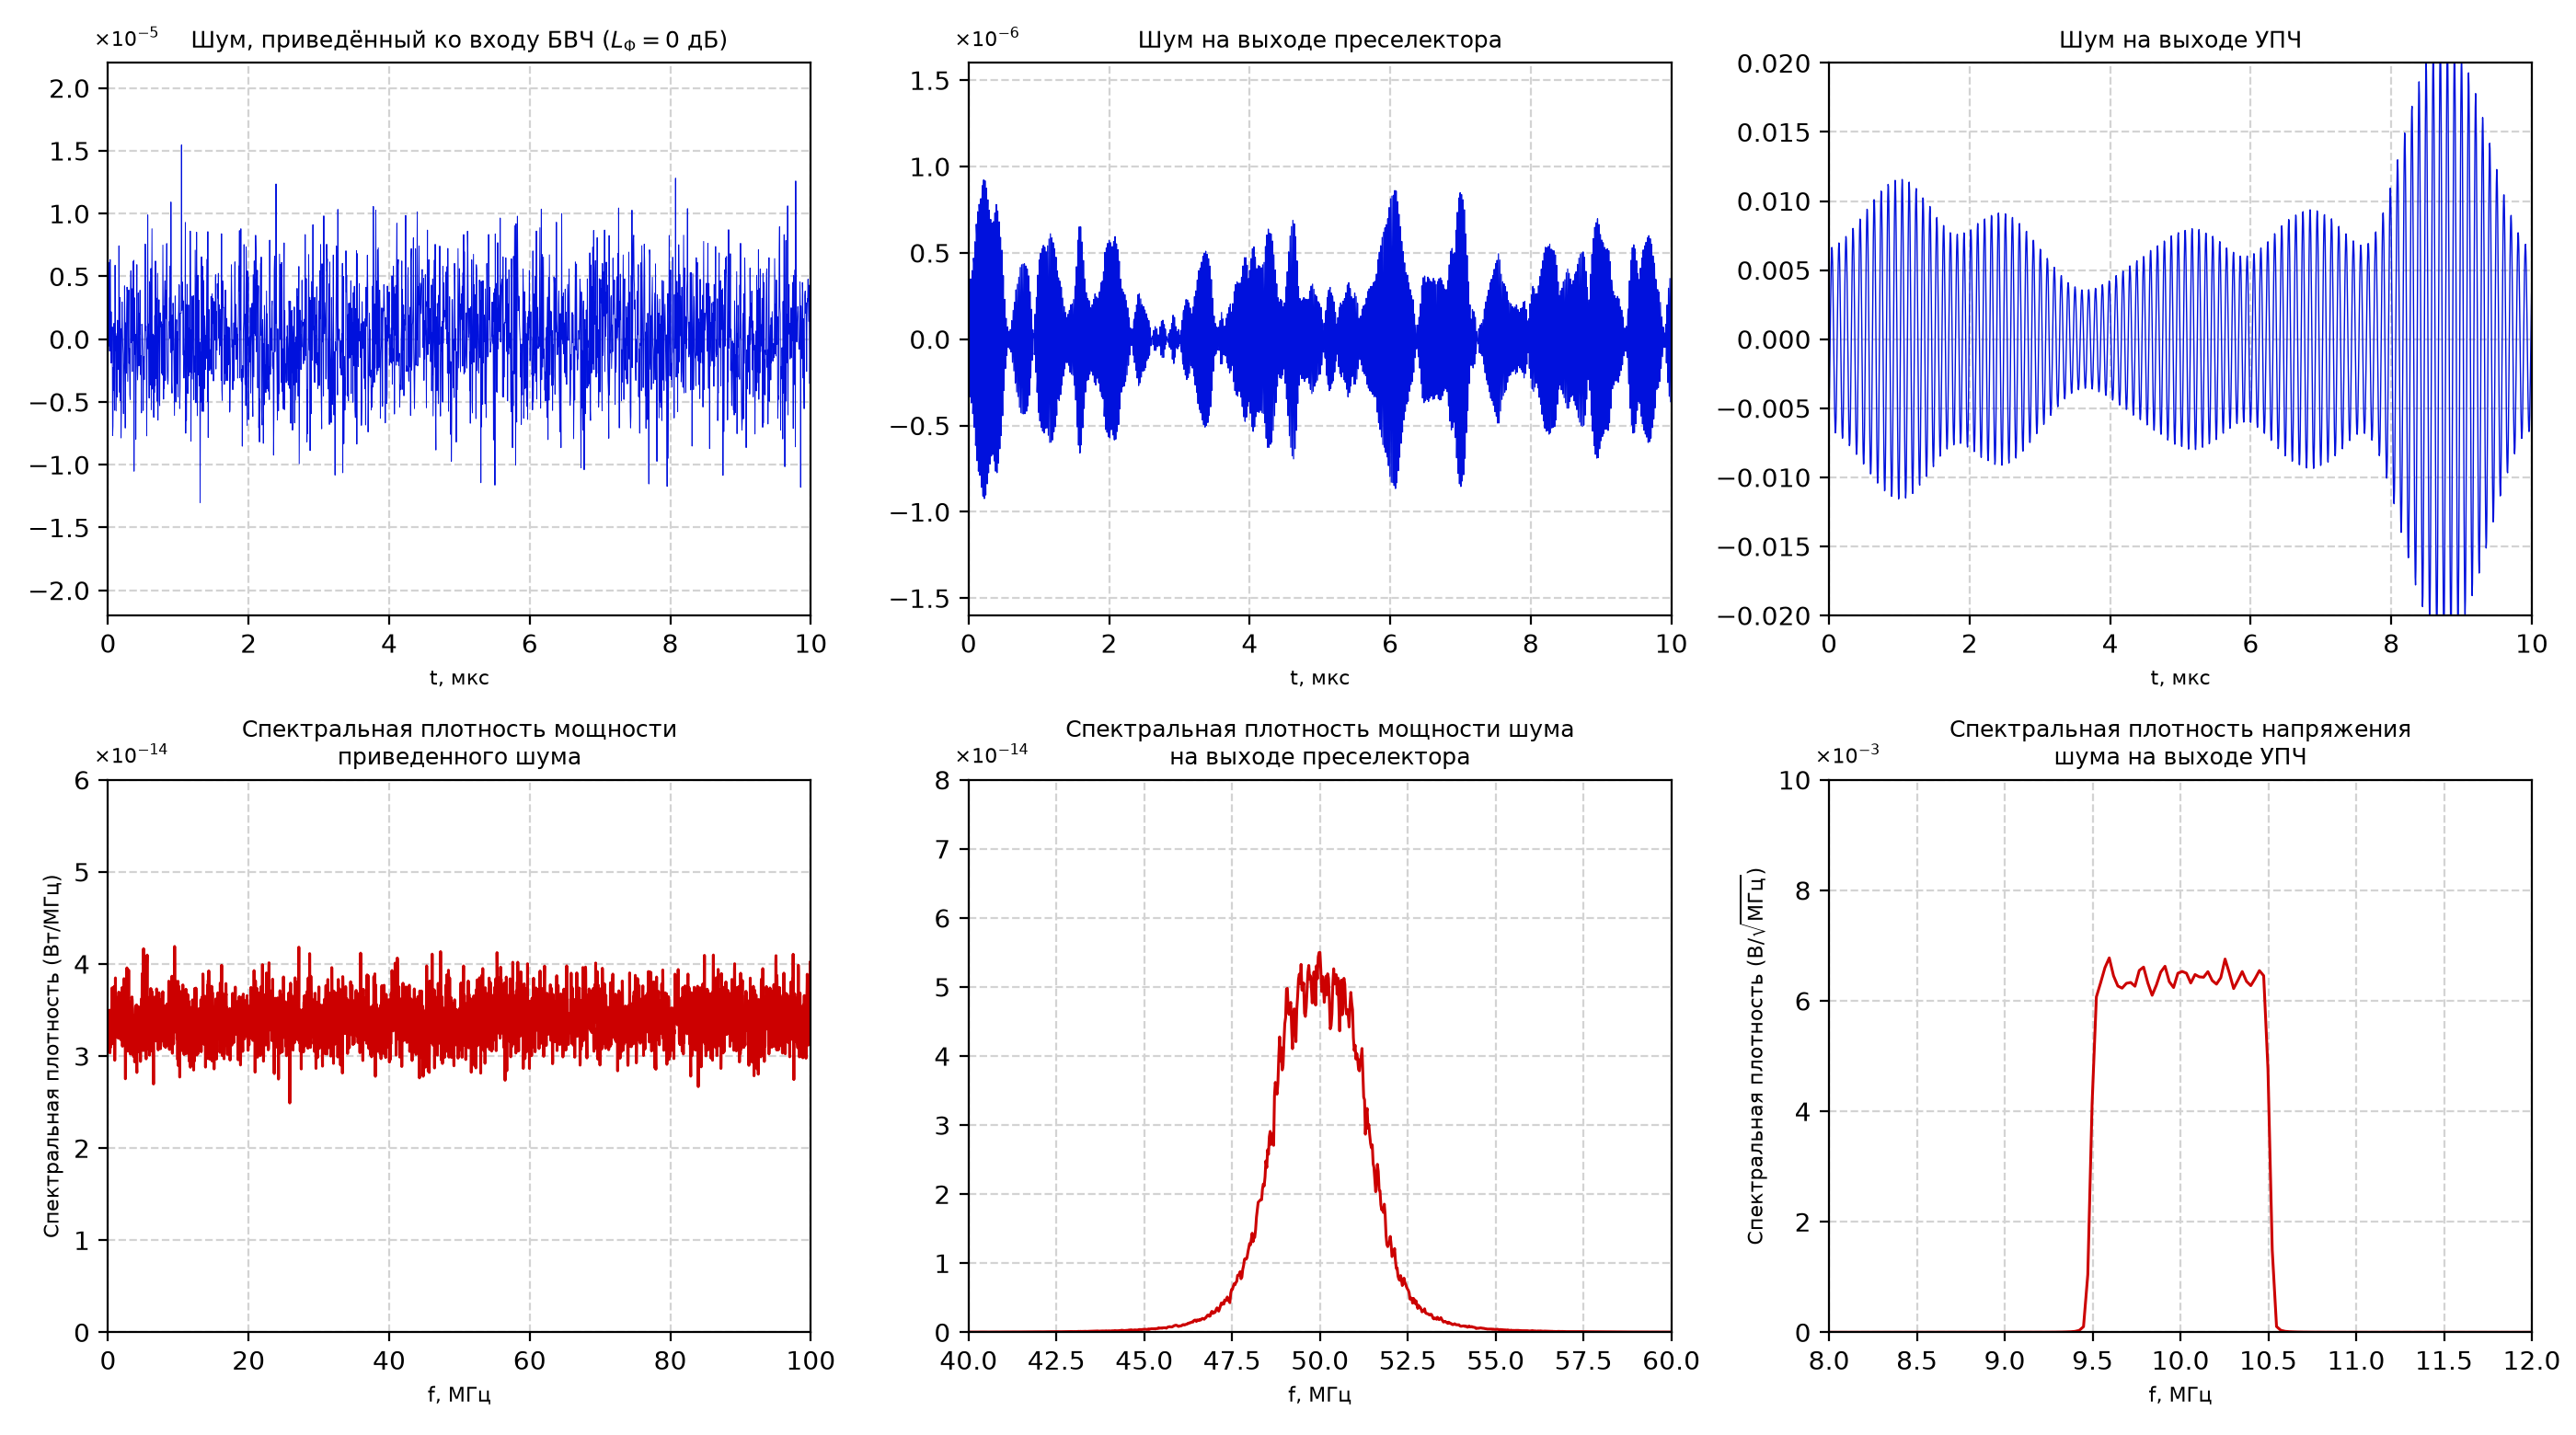
\includegraphics[width=0.98\linewidth]{exports_fig/pic6.png}
    \caption{Характеристики шума в тракте БВЧ при отсутствии потерь в фидере ($L_\Phi = 0$~дБ)}
    \label{fig:pic6}
\end{figure}

Устранение потерь в фидере уменьшает сквозной шум тракта за счёт исключения собственного шума пассивного четырехполюсника и отсутствия ослабления сигнала перед первым усилителем. СПМ приведённого шума снижается с $4{,}26 \cdot 10^{-14}$ до $3{,}39 \cdot 10^{-14}$~Вт/МГц, что приводит к повышению чувствительности РПУ примерно на $1$~дБ. Однако выигрыш оказывается менее выраженным, чем при увеличении коэффициента передачи преселектора или снижении шума смесителя, поскольку в исходной схеме основной вклад в $K_{\text{ш БВЧ}}$ вносили последующие активные каскады.



\subsection{Расчёт характеристик шума в различных точках приёмного тракта}

Выполним аналитический расчёт параметров шума в контрольных сечениях тракта БВЧ при номинальном режиме работы и сопоставим их со значениями, зафиксированными на модели. Точки анализа соответствуют схеме БВЧ (Рис.~\ref{fig:scheme_bvch}): сечение \textbf{2} — выход преселектора, сечение \textbf{3} — выход УПЧ.

Максимальное значение спектральной плотности мощности шума на выходе преселектора определяется коэффициентом передачи предшествующих звеньев:
\begin{equation}
    G_{\text{ш.прес. max}} = G_{\Sigma\text{ ном}}' \cdot K_{p\Phi} \cdot K_{p\text{ прес}} = 4{,}257 \cdot 10^{-20} \cdot \frac{1{,}585}{1{,}26} \approx 5{,}36 \cdot 10^{-20}\text{ Вт/Гц}.
\end{equation}

Шумовая полоса двухконтурного преселектора с критической связью контуров при полосе пропускания $\Pi_{\text{прес}} = 3$~МГц рассчитывается по формуле:
\begin{equation}
    \Pi_{\text{ш.прес}} = \frac{\pi}{4\sqrt{\sqrt{2}-1}}\,\Pi_{\text{прес}} \approx 1{,}220 \cdot 3 \cdot 10^6 \approx 3{,}66 \cdot 10^6\text{ Гц}.
\end{equation}

Тогда полная мощность шума на выходе преселектора составляет:
\begin{equation}
    P_{\text{ш.прес}} = G_{\text{ш.прес. max}} \cdot \Pi_{\text{ш.прес}} = 5{,}36 \cdot 10^{-20} \cdot 3{,}66 \cdot 10^6 \approx 1{,}96 \cdot 10^{-13}\text{ Вт}.
\end{equation}

По графику спектральной плотности шума на выходе преселектора (Рис.~\ref{fig:bvch_simulation_base}) ширина спектра по уровню половинной мощности $0{,}5$ составляет $\Delta f_{0{,}5} \approx 3{,}0$~МГц (интервал от $48{,}5$ до $51{,}5$~МГц), что строго совпадает с заданной полосой пропускания фильтра $\Pi_{\text{прес}} = 3$~МГц.

Шум с выхода преселектора проходит через смеситель (ПЧ) с коэффициентом передачи мощности $K_{p\text{ ПЧ}} = 1{,}995$. Спектральная плотность мощности шума на входе УПЧ равна:
\begin{equation}
    G_{\text{ш.пч}} = G_{\text{ш.прес. max}} \cdot K_{p\text{ ПЧ}} = 5{,}36 \cdot 10^{-20} \cdot 1{,}995 \approx 1{,}069 \cdot 10^{-19}\text{ Вт/Гц}.
\end{equation}

На согласованном входном сопротивлении УПЧ $R_{\text{вх.УПЧ}} = 50$~Ом спектральная плотность квадрата напряжения шума принимает вид:
\begin{equation}
    G_{U\text{ ш.пч}}^2 = G_{\text{ш.пч}} \cdot R_{\text{вх.УПЧ}} = 1{,}069 \cdot 10^{-19} \cdot 50 \approx 5{,}35 \cdot 10^{-18}\text{ В}^2/\text{Гц}.
\end{equation}

С учётом коэффициента усиления тракта УПЧ по напряжению $K_0 = 3000$ максимальное значение спектральной плотности дисперсии шума на выходе составляет:
\begin{equation}
    G_{U\text{ ш.упч max}}^2 = G_{U\text{ ш.пч}}^2 \cdot K_0^2 = 5{,}35 \cdot 10^{-18} \cdot 3000^2 \approx 4{,}81 \cdot 10^{-11}\text{ В}^2/\text{Гц}.
\end{equation}

Эквивалентная шумовая полоса пропускания тракта УПЧ определяется частотной характеристикой избирательной цепи ($\Pi_{\text{упч}} = 1$~МГц):
\begin{equation}
    \Pi_{\text{ш.упч}} = \frac{\pi}{2} \Pi_{\text{упч}} = \frac{\pi}{2} \cdot 10^6 \approx 1{,}57\text{ МГц}.
\end{equation}

Эффективное напряжение шума на выходе УПЧ при полосе пропускания $\Pi_{\text{УПЧ}} = 1$~МГц равно:
\begin{equation}
    U_{\text{ш.упч}} = \sqrt{G_{U\text{ ш.упч max}}^2 \cdot \Pi_{\text{УПЧ}}} = \sqrt{4{,}81 \cdot 10^{-11} \cdot 10^6} \approx 6{,}93 \cdot 10^{-3}\text{ В} \approx 6{,}93\text{ мВ}.
\end{equation}

Сведём теоретически рассчитанные величины и данные, полученные на виртуальном стенде, в Таблицу~\ref{tab:comparison_bvch}.

\begin{table}[H]
\centering
\caption{Сравнение расчётных и экспериментальных характеристик шума БВЧ}
\label{tab:comparison_bvch}
\begin{tabular}{|l|c|c|c|}
\hline
\textbf{Параметр} & \textbf{Расчёт} & \textbf{Модель} & \textbf{Погрешность} \\ \hline
$G_{\Sigma\text{ ном}}'$, Вт/Гц & $4{,}26 \cdot 10^{-20}$ & $4{,}26 \cdot 10^{-20}$ & $< 0{,}1\%$ \\ \hline
$G_{\text{ш.прес. max}}$, Вт/Гц & $5{,}36 \cdot 10^{-20}$ & $5{,}30 \cdot 10^{-20}$ & $1{,}1\%$ \\ \hline
$P_{\text{ш.прес}}$, Вт & $1{,}96 \cdot 10^{-13}$ & $1{,}94 \cdot 10^{-13}$ & $1{,}0\%$ \\ \hline
$G_{U\text{ ш.упч max}}^2$, В$^2$/Гц & $4{,}81 \cdot 10^{-11}$ & $4{,}22 \cdot 10^{-11}$ & $12{,}3\%$ \\ \hline
$U_{\text{ш.упч}}$, мВ & $6{,}93$ & $6{,}41$ & $7{,}5\%$ \\ \hline
\end{tabular}
\end{table}

Результаты численного моделирования подтверждают высокую точность аналитических расчётов характеристик шума по тракту (погрешность мощности шума преселектора не превышает $1\%$). Незначительное расхождение в эффективном напряжении на выходе УПЧ обусловлено неидеальностью прямоугольной формы АЧХ реального тракта и статистической погрешностью оценки дисперсии. Измеренная ширина спектра шума на выходе преселектора по уровню $0{,}5$ совпадает с заданной полосой пропускания $\Pi_{\text{прес}} = 3$~МГц.

\subsection{Характеристики шума на выходе ФСС}

Рассчитаем номиналы элементов фильтра (индуктивностей и ёмкостей) для 8-го варианта ($f_{\text{п}} = 10$~МГц, $\Pi_{\text{ФСС}} = 0{,}55$~МГц, $\rho = 2{,}8$~кОм) по формулам методического пособия

\begin{align*}
    C_{\text{св}} &= \frac{1}{2\pi f_{\text{п}} \rho} = \frac{1}{2\pi \cdot 10^7 \cdot 2800} \approx 5{,}684\text{ пФ}, \\
    C_2 &= \frac{1}{\pi \Pi_{\text{ФСС}} \rho} - 2C_{\text{св}} = \frac{1}{\pi \cdot 0{,}55 \cdot 10^6 \cdot 2800} - 2 \cdot 5{,}684 \cdot 10^{-12} \approx 191{,}667\text{ пФ}, \\
    C_1 &= \frac{C_2}{2} = \frac{191{,}667}{2} \approx 95{,}833\text{ пФ}, \\
    L_2 &= \frac{\Pi_{\text{ФСС}} \rho}{4\pi f_{\text{п}}^2} = \frac{0{,}55 \cdot 10^6 \cdot 2800}{4\pi \cdot (10^7)^2} \approx 1{,}225\text{ мкГн}, \\
    L_1 &= 2 L_2 = 2 \cdot 1{,}225 \approx 2{,}450\text{ мкГн}.
\end{align*}

Полученные значения номиналов (с соблюдением точности не менее трёх знаков после запятой) вводятся в схему модели ФСС. 
\begin{figure}[H]
    \centering
    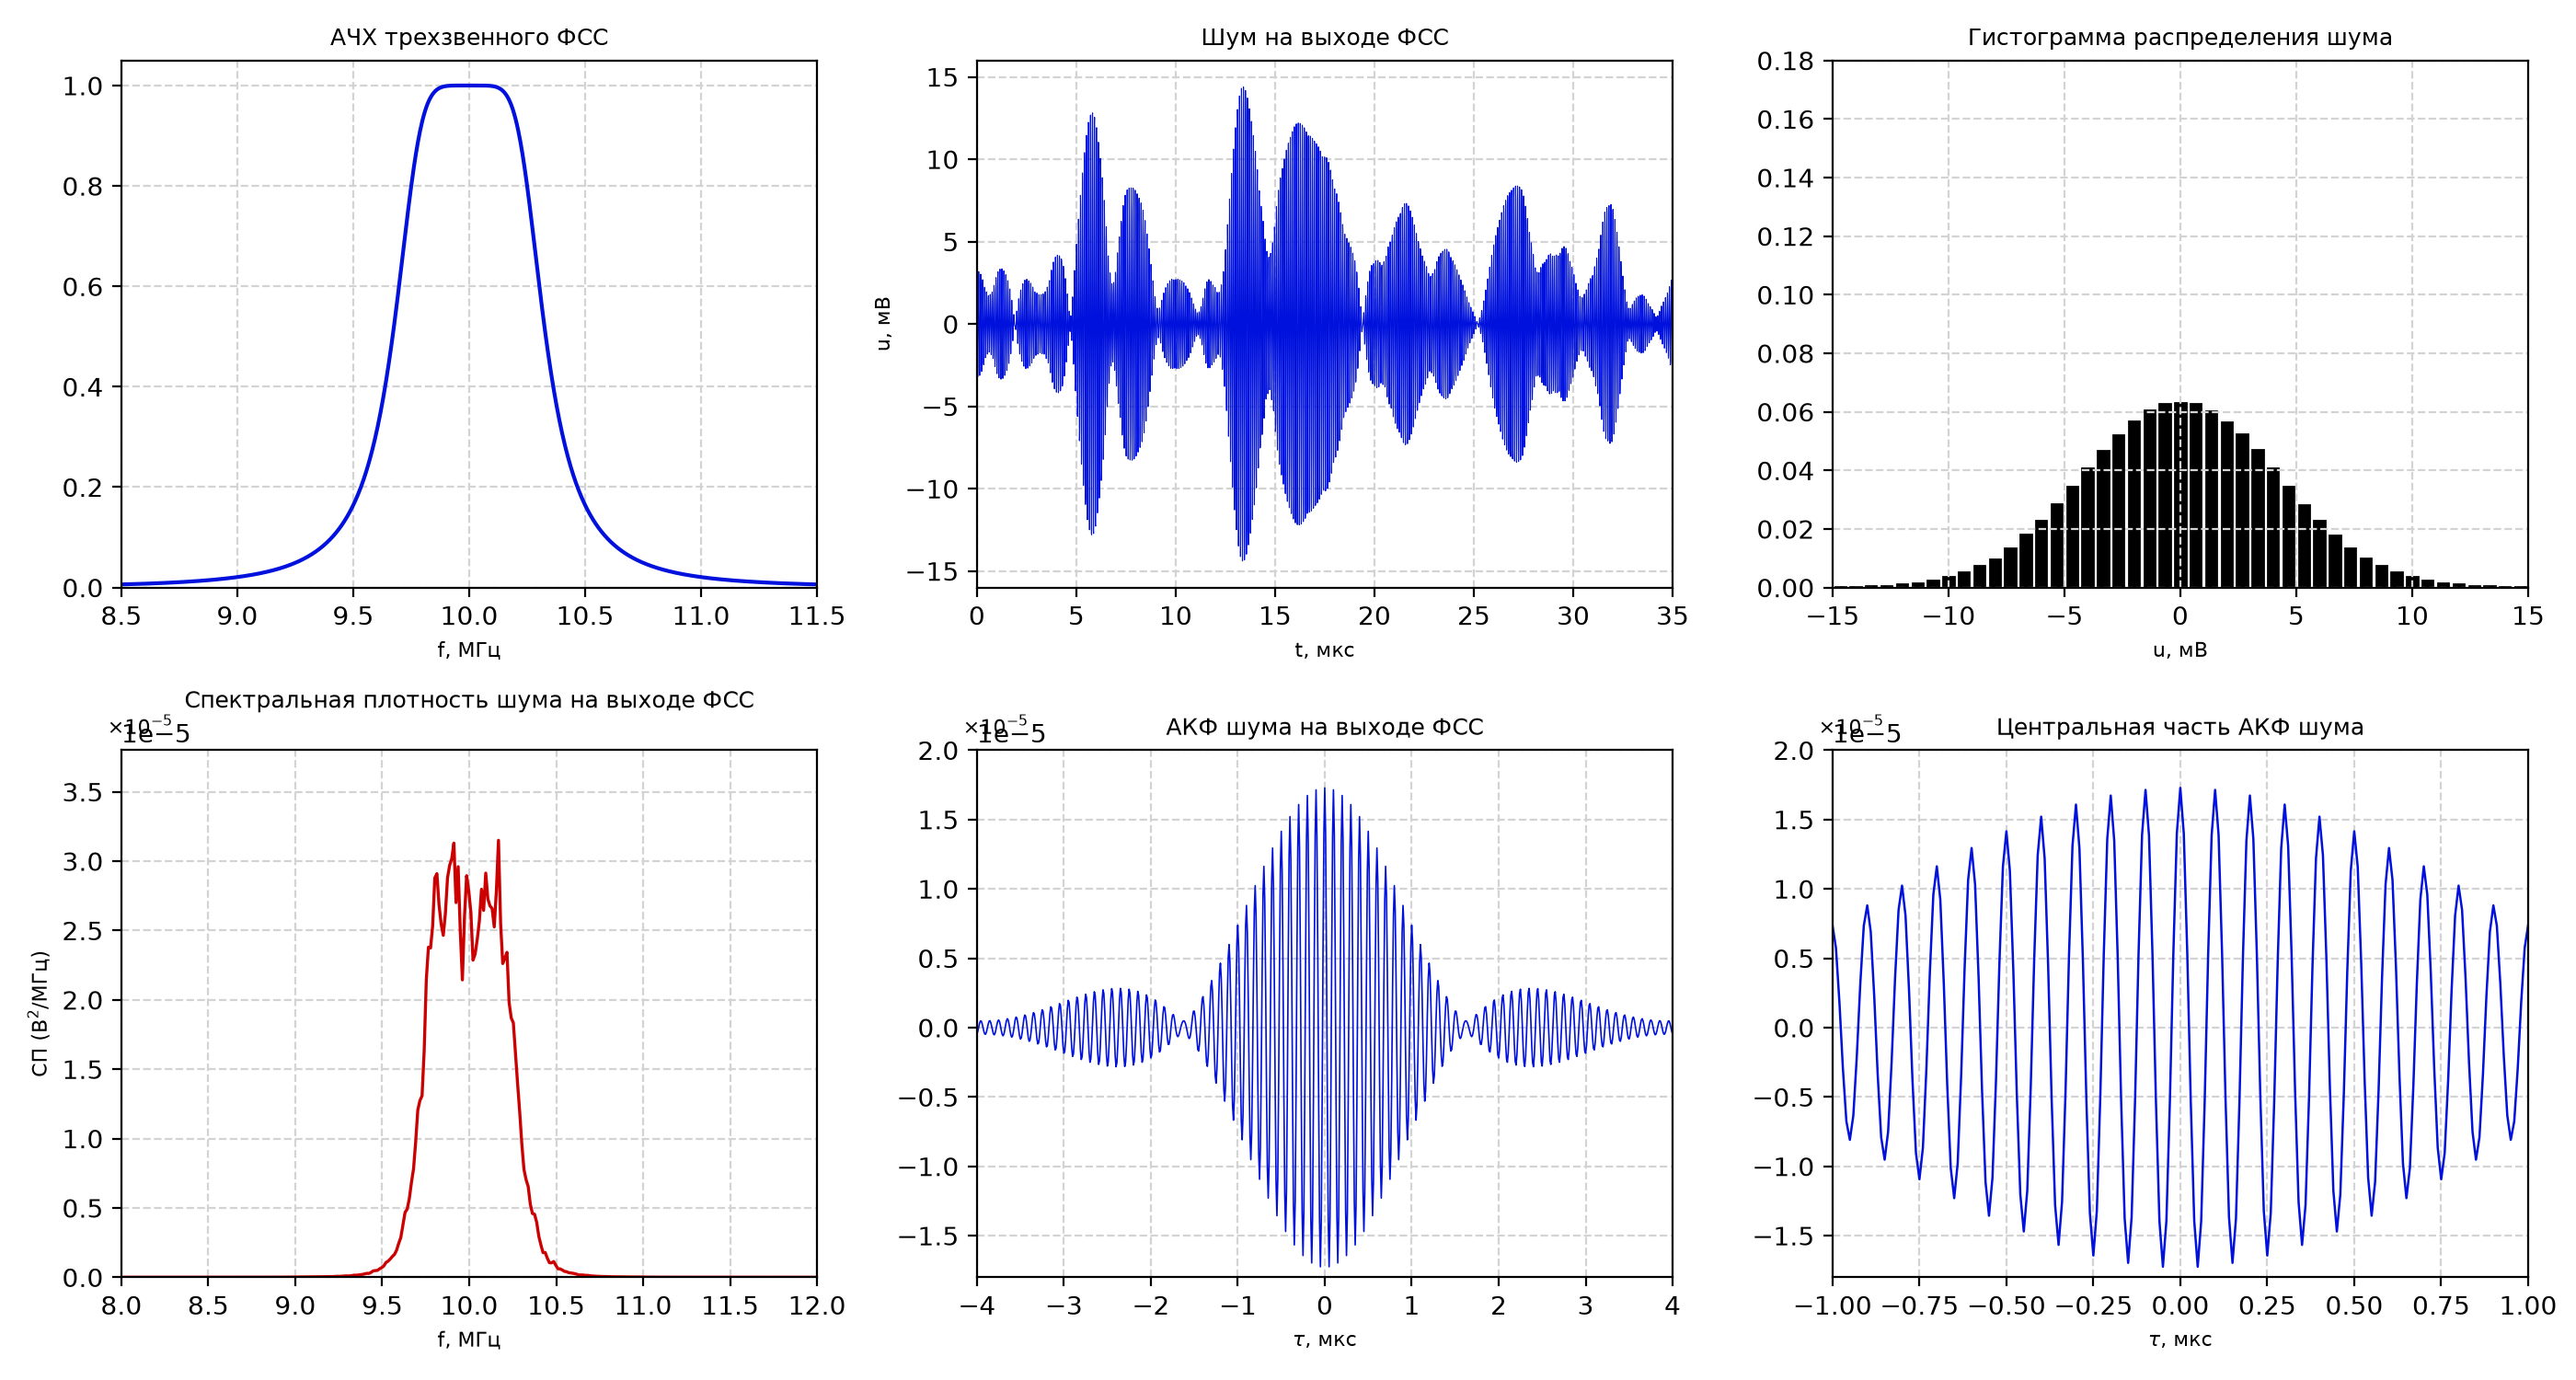
\includegraphics[width=0.98\linewidth]{exports_fig/pic_fss_results.png}
    \caption{Результаты моделирования характеристик трёхзвенного ФСС (8-й вариант)}
    \label{fig:fss_results}
\end{figure}
По результатам имитационного моделирования на стенде получены следующие характеристики:
\begin{itemize}
    \item АЧХ фильтра имеет симметричную колоколообразную форму с максимумом на центральной частоте $10$~МГц и полосой по уровню $0{,}5$, равной $\Pi_{\text{ФСС}} = 0{,}55$~МГц.
    \item Эффективное напряжение шума на выходе ФСС составляет $U_{\text{ш.фсс}} \approx 2{,}34$~В (или мВ в зависимости от масштаба вольтметра на стенде).
    \item Спектральная плотность дисперсии шума, гистограмма и автокорреляционная функция (АКФ) подтверждают стационарность и узкополосный характер процесса на выходе фильтра.
\end{itemize}
